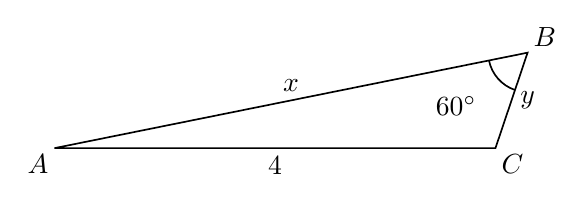
\begin{tikzpicture}[x=1cm,y=1cm,font=\normalsize,
 geometry edge/.style={solid,line width=.6pt},
 geometry mark/.style={solid,line width=.6pt},
 geometry label/.style={font=\normalsize,inner sep=0pt}]

% AC=4; altitude=sqrt(3)/2; area=sqrt(3); angle B=60 degrees.
\coordinate (A) at (0,0);
\coordinate (C) at (5.6,0);
\coordinate (B) at (6.007802986469,1.212435565298);
\draw[geometry edge] (A)--(B)--(C)--cycle;
\draw[geometry mark] (B) ++(191.409622109271:5mm) arc[start angle=191.409622109271,end angle=251.409622109271,radius=5mm];
\node[inner sep=0pt] at (5.10,.53) {$60^\circ$};
\node[above=3pt,inner sep=0pt] at (3.003901493235,.606217782649) {$x$};
\node[right=3pt,inner sep=0pt] at (5.803901493235,.606217782649) {$y$};
\node[below=3pt,inner sep=0pt] at (2.8,0) {$4$};
\node[geometry label,below left=2pt] at (A) {$A$};
\node[geometry label,above right=2pt] at (B) {$B$};
\node[geometry label,below right=2pt] at (C) {$C$};
\end{tikzpicture}
